\section{Infraestrutura}

\subsection{Arquitetura}

Para o problema proposto foi desenhada uma infraestrutura capaz de responder às exigências descritas no enunciado, isto é, ser escalável e não ter pontos únicos de falha. Assim sendo, a arquitectura que é mais adequada é representada na próxima imagem.

\begin{figure}[!h]
\centering
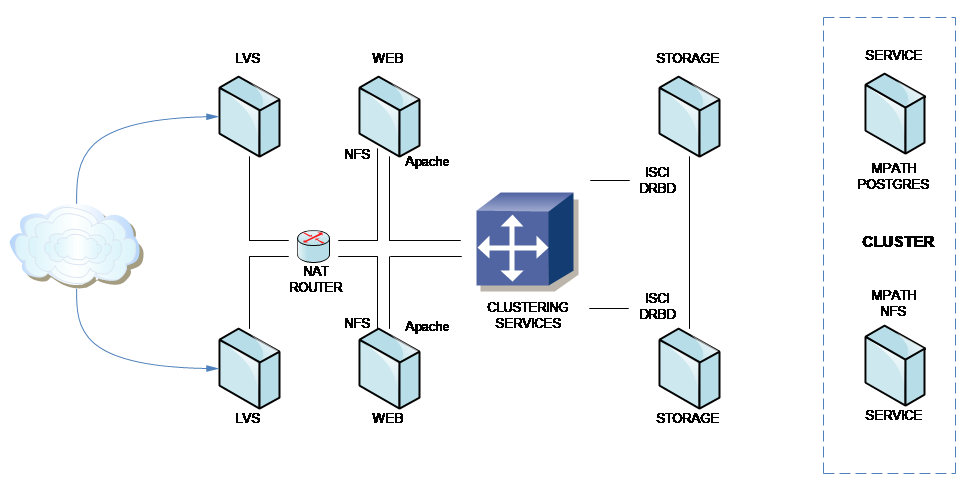
\includegraphics[scale=.6]{img/estrutura.png}
\caption{Arquitectura da Infraestrutura}
\end{figure}

Com o objetivo de se distribuir carga pelo sistema foi introduzida a componente \textit{LVS (Load Balancer)}, que é responsável por receber todos os pedidos do exterior e encaminhá-los por uma rede privada, sem acesso pelos utilizadores, até um \textit{WEB Server}. Este serviço está ligado a um \textit{Cluster} que contém os serviços para garantir alta disponibilidade e abstrair uma camada do \textit{Storage}.

Os componentes que foram implementados em cada serviço são descritos na próximas secções.

\subsection{Storage}
Esta componente é responsável por garantir alta disponibilidade e lidar com a persistência, quer nas máquinas, quer nos discos que a compõem. Tendo em conta o que foi dito anteriormente optou-se por colocar em um disco para persistência de dados os dados da base de dados.


Para tratar cada disco optou-se por duas máquinas que contém os serviços DRBD e \textit{iSCSI}. O primeiro serviço simula dois \textit{RAID1}, onde a característica é a replicação de dados, que no futuro, além da disponibilidade em caso de falha, torna-se bastante útil nas leituras de disco. O segundo serviço é responsável por permitir o acesso estes discos remotamente, através de \textit{TCP/IP}, que usufrui do armazenamento de dados que o serviço anterior oferece.

\subsection{Cluster}
O \textit{Cluster} é uma componente essencial nesta infraestrutura devido à garantia que fornece quanto à alta disponibilidade. Este é composto por três serviços, o \textit{PostgreSQL}, \textit{NFS Server} e \textit{Multipath} garantindo assim a disponibilidade inicialmente em duas máquinas e em caso de alguma falhar, então os serviçoes vão correr em menos uma das máquinas, o que provocará uma redução ao nível de desempenho, mas sem nunca perder os serviços, pois o \textit{Cluster} pode agir quando houver informarções que tal aconteciemento se sucedeu.

\subsection{WEB}
Esta componente apenas vai receber e atender os pedidos que chegam do exterior através do \textit{Load Balancer}, ou seja, contêm o serviço httpd para interpretar os pedidos e o NFS Cliente, que se liga ao NFS Server do \textit{Cluster} em execução, onde este terá acesso aos ficheiros que necessita para a interpretação e resposta do pedido.

O projeto Graphite é um sistema de gráficos em tempo real altamente escalável. Os dados podem ser visualizados através de interfaces web do Graphite.

\subsection{LVS}
Para garantir que a infraestrutura é estável e segura, foi necessário usar algo que fizesse a distribuição de carga pelos servidores da componente WEB. Assim, foram definidas duas máquinas com serviços para o tratamento dos pedidos. Para além da distribuição de carga que estes servidores conseguem efetuar, protegem ainda a infraestrutura do mundo exterior, nomeadamente através de um Virtual IP, por onde os clientes acedem ao serviço, acabando por filtrar os pedidos que não são esperados pela infraestrutura, originando assim, uma maior segurança.

O \textit{Load Balancer} fica entre o mundo exterior e dois (ou mais) servidores WEB que contém o mesmo conteúdo. Se um deles ficar em baixo, todos os pedidos serão automaticamente reencaminhados para o servidor WEB restante. Significa que, os utilizadores nunca notarão qualquer interrupção no serviço.
